\section {Two bits out of three using one (Information theory)}
You need to setup a communication protocol to transport $3$ bits at a time. Whenever you are given three bits of information you may only pass one bit over the medium to represent that information. The receiver should be able to produce the $3$ bits with a maximum of 1 bit of mistake (anywhere).

\subsection{Solution}
If we put all $8$ possible $3$ bit combinations in a graph where two combinations are connected via an edge iff there is just 1 bit of information difference between them we see that $000$ and $111$ are at the edges of the graph and are $1$ bit close to $001, 010, 100$ and $011, 101 110$ respectively. This means that the entire group of $8$ possibilities could be divided into $2$ groups of $4$ thus: $000, 001, 010, 100$ and $111, 011, 101, 110$. So when we get $3$ bits of information we will send $0$ for any member of the first group and $1$ for any member of the second. The receiver will guess $000$ for $0$ and $111$ for $1$. This means that the receiver will be wrong by at most $1$ bit. The chance that the receiver will get the 3rd bit right is 1 in 4 if the input is evenly distributed. We can also reverse the meaning of $0$ and $1$ and have the decoder guess $111$ for $0$ and $000$ for $1$. Actually we are sending $0$ when most bits are $0$ and $1$ when most bits are $1$ and since most out of $3$ is at least $2$ we always get $2$ bits right. Note that we can't choose other representatives for the groups, and not even representatives which are reverse of each other (like $001$ and $110$) since these are not distanced by at most $1$ bit from the rest of the group that they are in (for instance $001$ has distance $2$ from $100$).

\begin{center}
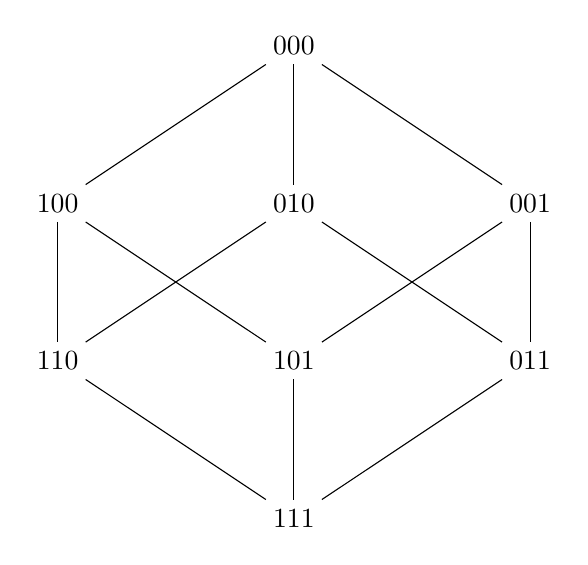
\begin{tikzpicture}
\node (000) at (12,10) {000};
\node (001) at (15,8) {001};
\node (010) at (12,8) {010};
\node (100) at (9,8) {100};
\node (011) at (15,6) {011};
\node (101) at (12,6) {101};
\node (110) at (9,6) {110};
\node (111) at (12,4) {111};

\foreach \from/\to in {000/001,000/010,000/100,010/011,010/110,001/011,001/101,111/011,111/110,111/101,100/110,100/101}
\draw (\from) -- (\to);
\end{tikzpicture}
\end{center}

If we look at the graph then we see that any bi-partition of the graph would work as well. For instance we could divide the graph to $001, 000, 101, 011$ and $110, 100, 010, 111$. The first group the representative will be $001$ and the second group representative will be $110$. Actually the graph is so symmetric that any two negative bitwise strings would do to partition it so there are $4$ possible protocols ($8$ if reverse counts too).
